% AY2016 制御工学 解答例
% 回答の流れ・言葉遣いは 03_制御工学/参考/「制御工学Ⅱ（完成版）」に寄せる。
% デザイン（囲み枠等）は真似しない。解答・数値は本年度過去問から自力で導いた。
\documentclass[11pt,a4paper]{article}
\usepackage{../../../00_common/preamble}

\usetikzlibrary{positioning,arrows.meta,calc}
\usepackage{pgfplots}
\pgfplotsset{compat=newest}

\title{制御工学 AY2016 解答例（専門応用科目I）}
\author{}
\date{}

\begin{document}
\maketitle

% ==================================================================
\section*{第1問〔I〕}

壁 $-$ バネ $k$ $-$ 質量 $m$ $-$ ダンパ $d$ $-$ 自由端（入力 $x_1$）の振動系。$x_2$ は質量の変位。

\subsection*{(1) 伝達関数}
バネは壁と質量を、ダンパは質量と自由端を結ぶ。質量の運動方程式は
\begin{align*}
  &\qquad m\ddot{x}_2=-k x_2+d(\dot{x}_1-\dot{x}_2)\\
  &\therefore\quad m\ddot{x}_2+d\dot{x}_2+k x_2=d\dot{x}_1\\
  &\therefore\quad (ms^2+ds+k)X_2(s)=ds\,X_1(s).
\end{align*}
\[
  \therefore\quad \ans{\;G(s)=\dfrac{X_2(s)}{X_1(s)}=\dfrac{ds}{ms^2+ds+k}\;}
\]

\subsection*{(2) ステップ応答（$m=1,d=3,k=2$）}
$G(s)=\dfrac{3s}{s^2+3s+2}=\dfrac{3s}{(s+1)(s+2)}$。$X_1(s)=\dfrac1s$ より
\begin{align*}
  &\qquad X_2(s)=\frac{3s}{(s+1)(s+2)}\cdot\frac1s=\frac{3}{(s+1)(s+2)}
   =\frac{3}{s+1}-\frac{3}{s+2}\\
  &\therefore\quad x_2(t)=3\bigl(\e^{-t}-\e^{-2t}\bigr).
\end{align*}
分子に $s$ をもつ（$s=0$ に零点）ため直流ゲインは $0$。よって定常値は $0$。
\[
  \therefore\quad \ans{\;x_2(t)=3(\e^{-t}-\e^{-2t}),\qquad x_2(\infty)=0\;}
\]

\subsection*{(3) 最大値と発生時間}
\begin{align*}
  &\qquad \dot{x}_2(t)=3(-\e^{-t}+2\e^{-2t})=0
   \quad\therefore\quad 2\e^{-2t}=\e^{-t}\\
  &\therefore\quad \e^{t}=2
   \quad\therefore\quad t=\ln 2.
\end{align*}
このとき $x_2=3\bigl(\tfrac12-\tfrac14\bigr)=\tfrac34$。
\[
  \therefore\quad \ans{\;x_{2\max}=\dfrac34\ \ (t=\ln2\approx0.69)\;}
\]

\subsection*{(4) $k=0$ の場合（$m=1,d=3,k=0$）}
\begin{align*}
  &\qquad G(s)=\frac{3s}{s^2+3s}=\frac{3s}{s(s+3)}=\frac{3}{s+3}\\
  &\therefore\quad X_2(s)=\frac{3}{s(s+3)}=\frac1s-\frac{1}{s+3}
   \quad\therefore\quad x_2(t)=1-\e^{-3t}.
\end{align*}
$k=0$ では $G(0)=1$ となり、定常値は $1$（バネがないため自由端の変位がそのまま質量に伝わる）。
\[
  \therefore\quad \ans{\;x_2(t)=1-\e^{-3t},\qquad x_2(\infty)=1\;}
\]

\bigskip
\noindent 検算: (2) は $G$ が $s=0$ に零点をもち定常 $0$、(3) は $t=\ln2$ で $x_{2\max}=\tfrac34$、
(4) は $G=3/(s+3)$ で定常 $1$ を SymPy で確認✓。

\newpage
% ==================================================================
\section*{第2問〔II〕}

$G_1,G_2,G_3$ を直列にし、$G_2$ の出力を $G_2$ 入力側へ（内側）、$G_2$ 入力点を入力側へ（外側）
それぞれ負帰還した系を考える。

\subsection*{(1) 伝達関数}
$G_2$ 入力（$=$ sum2 出力）を $a$ とおく。内側帰還より $a=G_1(\cdots)-G_2 a$、
外側帰還より $G_1$ 入力 $=U-a$。整理すると
\begin{align*}
  &\qquad a(1+G_2)=G_1(U-a)
   \quad\therefore\quad a(1+G_1+G_2)=G_1 U\\
  &\therefore\quad Y=G_3 G_2\,a=\frac{G_1G_2G_3}{1+G_1+G_2}\,U.
\end{align*}
\[
  \therefore\quad \ans{\;\dfrac{Y}{U}=\dfrac{G_1G_2G_3}{1+G_1+G_2}\;}
\]

\subsection*{(2) ゲインとゲイン線図（$G_1=\frac3s,\ G_2=\frac{1}{s+4},\ G_3=4$）}
\begin{align*}
  &\qquad \frac{Y}{U}=\frac{\frac3s\cdot\frac{1}{s+4}\cdot4}{1+\frac3s+\frac{1}{s+4}}
   =\frac{12/(s(s+4))}{(s^2+8s+12)/(s(s+4))}
   =\frac{12}{(s+2)(s+6)}.
\end{align*}
ゲインは $s=j\omega$ として
\[
  \therefore\quad \ans{\;R=|T(j\omega)|=\dfrac{12}{\sqrt{(12-\omega^2)^2+(8\omega)^2}}\;}\qquad(R|_{\omega=0}=1=0\,\mathrm{dB})
\]
時定数形 $\dfrac{1}{(1+s/2)(1+s/6)}$ より折れ点は $\omega=2,\ 6$、傾きは $\omega<2$ で $0$、
$2<\omega<6$ で $-20$、$\omega>6$ で $-40\,[\mathrm{dB/dec}]$。

\begin{center}
\begin{tikzpicture}
\begin{axis}[
  width=0.86\linewidth, height=4.8cm,
  xmin=1e-1, xmax=1e3, ymin=-80, ymax=20, xmode=log,
  xlabel={$\omega\,[\mathrm{rad/s}]$}, ylabel={ゲイン [dB]},
  ytick={-80,-60,-40,-20,0,20},
  xmajorgrids=true, ymajorgrids=true, xminorgrids=true,
  grid style={line width=0.3pt, draw=gray!60},
  extra y ticks={0}, extra y tick style={grid=major, grid style={line width=1pt, draw=black}},
  legend pos=south west, clip=true, enlargelimits=false,
]
% (2): 折れ点 2,6
\addplot[thick] coordinates {(0.1,0) (2,0) (6,-9.5) (1000,-113.5)};
\addlegendentry{(2) $G_3=4$}
% (4): T=6/(s+6) 折れ点6のみ
\addplot[thick,dashed] coordinates {(0.1,0) (6,0) (1000,-44.4)};
\addlegendentry{(4) $G_3=2s+4$}
\node[anchor=south] at (axis cs:2,0) {\scriptsize $\omega=2$};
\node[anchor=south west] at (axis cs:6,0) {\scriptsize $\omega=6$};
\end{axis}
\end{tikzpicture}
\end{center}

\subsection*{(3) ステップ応答（(2)）}
極は実数 $s=-2,-6$（過減衰）。$X(s)=\dfrac{T(s)}{s}$ を部分分数分解して
\begin{align*}
  &\qquad X(s)=\frac{12}{s(s+2)(s+6)}
   =\frac{1}{s}-\frac{1.5}{s+2}+\frac{0.5}{s+6}\\
  &\therefore\quad x(t)=1-1.5\,\e^{-2t}+0.5\,\e^{-6t}.
\end{align*}
オーバーシュートなく単調に立ち上がり、定常値 $1$ に収束する。支配極は $s=-2$（時定数 $0.5\,$s）。
\[
  \therefore\quad \ans{\;x(t)=1-1.5\,\e^{-2t}+0.5\,\e^{-6t}\;}
\]

\begin{center}
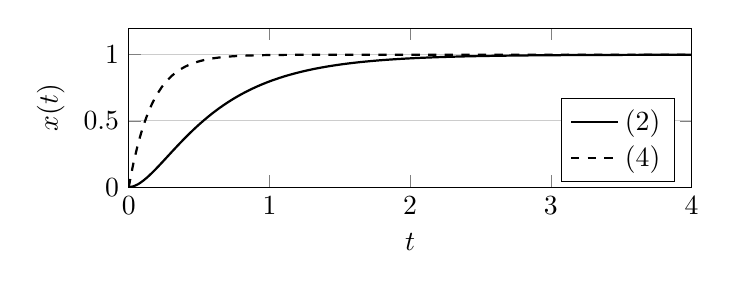
\begin{tikzpicture}
\begin{axis}[
  width=0.72\linewidth, height=3.6cm,
  xmin=0, xmax=4, ymin=0, ymax=1.2,
  xlabel={$t$}, ylabel={$x(t)$},
  ytick={0,0.5,1}, ymajorgrids=true, grid style={gray!40},
  legend pos=south east,
]
\addplot[thick,domain=0:4,samples=120]{1-1.5*exp(-2*x)+0.5*exp(-6*x)};
\addlegendentry{(2)}
\addplot[thick,dashed,domain=0:4,samples=120]{1-exp(-6*x)};
\addlegendentry{(4)}
\end{axis}
\end{tikzpicture}
\end{center}

\subsection*{(4) $G_3=2s+4$ の場合の比較}
$G_3=2s+4=2(s+2)$ とすると、分母 $1+G_1+G_2$ は変わらず分子だけ変化し
\begin{align*}
  &\qquad T(s)=\frac{\frac3s\cdot\frac{1}{s+4}\cdot2(s+2)}{1+\frac3s+\frac{1}{s+4}}
   =\frac{6(s+2)}{(s+2)(s+6)}=\frac{6}{s+6}.
\end{align*}
$G_3$ の零点 $s=-2$ が極 $s=-2$ を相殺し、1 次系になる。ステップ応答は
\[
  X(s)=\frac{6}{s(s+6)}=\frac1s-\frac{1}{s+6}
  \quad\therefore\quad \ans{\;x(t)=1-\e^{-6t}\;}
\]
\textbf{考察}：定常値はどちらも $1$ で不変。一方、過渡特性は次のように改善される。
\begin{itemize}\setlength{\itemsep}{1pt}
  \item \textbf{時間応答}：(2) は遅い極 $s=-2$（$\tau=0.5\,$s）が応答を支配したが、(4) では
        これが相殺され $s=-6$（$\tau=1/6\approx0.17\,$s）の 1 次系となり、整定が約 3 倍速い。
  \item \textbf{ゲイン線図}：(2) は折れ点 $\omega=2,6$ で最終傾き $-40\,$dB/dec だが、(4) は
        折れ点が $\omega=6$ のみ・傾き $-20\,$dB/dec となり、帯域が広がる（速い応答に対応）。
\end{itemize}

\bigskip
\noindent 検算: (2) $T=12/((s+2)(s+6))$、(3) ステップ応答単調増加で定常 $1$、
(4) は零点相殺で $T=6/(s+6)$、$x=1-\e^{-6t}$ を SymPy で確認✓。

\end{document}
